\chapter{Investigation of Interface Favourability} \label{chapter:computational_investigation}

A key step in training a MLI model is building a dataset of physically plausible and energetically reasonable heterostructures\cite{Di_Liberto2022-gz, Batzner2022-fd}.
Ideally, such a dataset would be generated entirely using DFT, but the cost of relaxing and evaluating thousands of configurations makes this impractical\cite{Rosen2022-pw, Schutt2018-xc, Rosen2022-pw}.
Instead, this chapter investigates whether an MLP, specifically the MACE model, can assist in rapidly generating and assessing interface structures before applying DFT.

The focus here is not to validate MLPs as a replacement for DFT, but to test their usefulness as part of a larger data-generation pipeline.
If MACE is able to help identify realistic and favourable structures, it can reduce the number of expensive DFT calculations needed and enable faster construction of training data for the MLI model.

The chapter is structured as follows: Section 1 describes the generation of the dataset, the chemical systems considered, and the use of ARTEMIS for constructing candidate interfaces.
Section 2 analyses how well the MACE model reproduces trends in DFT-calculated interface energetics.
Section 3 discusses and summarises analysis and findings.

\section{Methodology} \label{section:methodology}

The goal of this study is to support the development of an MLI model that can predict which heterostructures are likely to be realistic and favourable.
To train this model, we need a large dataset of physical interfaces that are not only valid in terms of their atomic arrangement but also low enough in energy to be found in real materials.
Relaxing and evaluating all possible interfaces using DFT would be too expensive, so we explore whether a Machine-Learned Potential (MLP), specifically MACE, can help us identify good candidates more efficiently.

Rather than replacing DFT, MACE is tested here as a screening tool: if MACE can roughly preserve the order of interface favourability that DFT gives, it could help us pick which interfaces to relax with DFT.
These comparisons are a means to an end, providing the MLI model with useful training data.

This work uses an iterative approach to building the dataset.
At each step, the number of materials, structures, and configurations is increased to explore broader behaviours and to identify issues in the workflow before scaling further.
Each iteration reflects what was possible with available computing resources and analysis at the time.
\begin{itemize}
    \item Iteration 1 focused on a small number of $Si|Ge$ interfaces generated and relaxed manually to test early code and analysis scripts.
    \item Iteration 2 expanded this to a much larger $Si|Ge$ dataset using automated tools like ARTEMIS, introducing slab shifting and filtering steps.
    \item Iteration 3, which forms the main dataset used in this chapter, includes materials from group $14$: carbon ($C$), silicon ($Si$), germanium ($Ge$), and tin ($Sn$).
\end{itemize}
These elements were chosen because they are widely used in electronics and all have four valence electrons, which avoids problems with charge imbalance when making interfaces.
Elements heavier than atomic number 83 are excluded to avoid needing relativistic corrections, it is also notable that MACE is trained on elements $Z \le 89$.

This third dataset uses a consistent generation workflow based on Miller plane selection, surface matching, and stacking with registry-aware shifts.
It avoids configurations with overlapping atoms and stores each system in a reproducible format for later energy evaluation.

\subsection{Interface Generation Protocol}

Interfaces were generated using the ARTEMIS toolkit (see \secref{sec:constructing_interfaces} for background on interface construction and lattice matching).
For each pair of materials, up to $64$ surface orientations (Miller planes) were explored to find possible ways the two materials could be stacked together.
ARTEMIS searched for matching supercells by expanding the unit cells of both materials up to $8 \times$ along the in-plane directions, looking for configurations with similar lattice vectors and angles (detailed in \secref{sec:lattice_mismatching}).
This helps distribute mismatch over more atoms and reduce the per-cell strain\cite{artemis_paper}.

A key goal in finding physically favourable interfaces is to minimise the energy penalties introduced by strain and unbonded valence electrons\cite{Gerber2023-yd, Butler2019-ws}.
Interfaces with large lattice mismatch or poor atomic registry often exhibit elevated formation energies due to elastic distortions or chemically unstable bonding environments\cite{Hepplestone2010-vw, Chagarov2015-ol, Zhang2016-lt}.
By contrast, coherent interfaces that exhibit low strain and high atomic registry are more likely to be energetically stable and experimentally realisable\cite{Gerber2023-yd, Davies2024-ju, Chagarov2015-ol}.

One strategy for achieving this is through supercell scaling\cite{artemis_paper}: we try to match lattice constants $a$ and $a'$ of two materials by finding integers $n$ and $m$ such that $n \cdot a \approx m \cdot a'$, distributing the residual mismatch over multiple unit cells (see discussion of supercell mismatch reduction in \secref{sec:lattice_mismatching}).
For example, silicon and germanium have lattice constants of $5.45\,\text{\AA{}}$ and $5.66\,\text{\AA{}}$, respectively.
Matching 22 unit cells of Si to 21 of Ge gives:
\begin{equation}
    |22 \cdot 5.45 - 21 \cdot 5.66| = 1.04~\text{\AA}
\end{equation}
which corresponds to a mismatch of approximately $0.047\,\text{\AA{}}$ per unit cell.
Scaling up to $2201 Si$ and $2119 Ge$ cells reduces this to:
\begin{equation}
    |2201 \cdot 5.45 - 2119 \cdot 5.66| = 1.91~\text{\AA} \quad \Rightarrow \quad \sim 0.0009~\text{\AA}~\text{mismatch per cell}
\end{equation}
Each increase in supercell size decreases the mismatch per unit cell by roughly an order of magnitude.

In addition to supercell scaling, the choice of interface orientation, described by Miller indices (explained in \secref{sec:orientation_matching}), can significantly influence atomic registry across the interface.
Each Miller plane represents a unique slice through the crystal lattice that exposes a specific atomic arrangement\cite{artemis_paper}.
By rotating, stacking, and aligning these planes between two different materials, one can search for surface combinations where atoms naturally align into coherent patterns.
ARTEMIS uses these surface alignments to explore many candidate configurations, seeking high registry where bonding across the interface is maximised and valence electrons are not left unpaired\cite{artemis_paper}.

Each matched interface was constructed from two slabs, each $6$ atomic layers thick, separated by a small vacuum gap.
ARTEMIS then applied systematic shifts in the $a$ and $b$ directions to explore stacking offsets between the slabs (details of which are discussed in \secref{sec:artemis_algorithm}).
Initially, zero-shift configurations were allowed, but these sometimes produced unphysical atomic overlaps along the $c$-axis.
These cases were filtered out during data cleaning.
Future datasets will attempt to reintroduce shift-zero configurations in $a$ and $b$ while borrowing $c$-axis separations from nearby stable interfaces.

Although ARTEMIS supports atomic swaps at the interface to explore alloy-like or disordered bonding environments\cite{artemis_paper}, this feature was not available in the version used for this study.
Such configurations will be generated in future iterations using the RAFFLE tool.

While ARTEMIS considered many potential surface combinations, only $29$ unique surfaces were ultimately included in the final dataset.
This reflects both the geometric constraints of lattice matching and the filtering applied to ensure physical plausibility of the generated structures.

All parts of the workflow, from building interfaces to reading the results, were automated using Python scripts.
This made it easier to run large numbers of calculations and keep track of everything.

Interfaces were generated and prepared for calculation using scripts that could run in bulk.
Each job was submitted to the compute cluster automatically.

Some calculations failed or gave broken outputs (like NaN energies).
These were filtered out automatically so they didn't affect the results.

The energy values from both MLP and DFT were read and stored in CSV files.
These files were used to calculate rankings and compare the methods.

\subsection{Ranking and Error Metrics}

To check how well the MLP results agree with DFT, we used a few simple measures.

\subsubsection*{Spearman $\rho$}

This checks if the overall order of interface energies is preserved between methods.
It compares the rankings and gives a score between $-1$ (completely reversed) and $1$ (perfect match):
\begin{equation}
    \rho = 1 - \frac{6 \sum d_i^2}{n(n^2 - 1)}
\end{equation}
Here $d_i$ is the difference in rank for the $i^\text{th}$ structure, and $n$ is the total number of structures.

\subsubsection*{Kendall $\tau$}
This checks whether pairs of structures are ranked in the same order between methods.
It also ranges from $-1$ to $1$:
\begin{equation}
    \tau = \frac{(\text{concordant pairs}) - (\text{discordant pairs})}{\frac{1}{2}n(n-1)}
\end{equation}

\subsubsection*{Top-N Overlap} his looks at how many of the best-ranked structures under DFT also appear in the top group under MLP. For example, how many of the top $5$ or top $10$ are shared.

\subsubsection*{Mean Absolute Error (MAE)} This shows the average difference in energy between MLP and DFT:
\begin{equation}
    \text{MAE} = \frac{1}{n} \sum_{i=1}^{n} |y_i - \hat{y}_i|
\end{equation}

\subsubsection*{Root Mean Square Error (RMSE)} This is another way of showing how different the energies are, giving more weight to large differences:
\begin{equation}
    \text{RMSE} = \sqrt{\frac{1}{n} \sum_{i=1}^{n} (y_i - \hat{y}_i)^2}
\end{equation}
These metrics help to determine whether the MLP is giving similar energy rankings and values to DFT, so it can be established whether it is useful for selecting structures for further study\nocite{}.

\subsection{Relaxation and Energy Evaluation}

In this study, the interface structures were not relaxed before comparing energies.
Instead, the same unrelaxed geometries were evaluated using both DFT and MLP to keep the comparison fair.
This helps isolate differences in energy prediction from differences caused by structural relaxation\cite{artemis_paper}.

DFT calculations were carried out using the VASP software.
Gamma-point sampling was used for simplicity and speed.
Calculations were limited to a $24$-hour walltime.
Structures that failed to complete were excluded from analysis.

The MACE model used here was the most recent release available at the time (downloaded in April 2025).
It was applied using the ASE library to compute total energies on the same unrelaxed structures as used for DFT.
No fine-tuning or delta-correction was applied.

While MLP-based relaxation was tested on some structures later in the workflow, those results were not used for ranking comparison in this section.
The goal is to test how well MLP can predict relative stability based on geometry alone.
DFT relaxations are planned for future datasets.

\section{Results and Analysis} \label{section:results_and_analysis}

This section presents the results of comparing unrelaxed DFT and MLP (MACE) energy rankings across $680$ valid heterostructures, grain boundaries, and alloyed systems involving the group 14 elements ($C$, $Si$, $Ge$, $Sn$).
The goal is to determine whether MACE, a machine-learned interatomic potential, can replicate DFT-derived rankings on unrelaxed geometries closely enough to serve as a pre-screening tool in the MLI data pipeline.

Across all evaluated systems, Spearman's rank correlation coefficient was extremely high:
\begin{equation}
    \rho = 0.9954, \qquad \tau = 0.9568
\end{equation}
This near-perfect alignment demonstrates that MACE preserves the order of interface favourability remarkably well, even without relaxation, suggesting strong potential as a filtering method for DFT candidate selection.

However, absolute energy agreement was poor:
\begin{equation}
    \text{RMSE} = 188.89~\text{eV}, \qquad \text{MAE} = 30.87~\text{eV}
\end{equation}
These large discrepancies reflect the fact that while MACE captures relative stability, its raw energy outputs are not quantitatively reliable without further training.
Despite this, the Top-$10$ overlap between DFT and MLP was $8/10$, indicating strong alignment in identifying favourable structures.

To understand how interface geometry impacts ranking fidelity, results were grouped into three categories: upper-slab heterostructures, lower-slab heterostructures, and homostructures (grain boundaries).
Average metrics across these categories are summarised in Table~\ref{tab:interface_metrics}.
\begin{table}
\centering
\caption{Average metrics for each interface type.}
\label{tab:interface_metrics}
\begin{tabular}{lrrrrrr}
\toprule
    Interface Type &   N &  Spearman $\rho$ &  Kendall $\tau$ &  RMSE (eV) &  MAE (eV) &  Top-10 Overlap \\
\midrule
\ce{C}|\ce{X} or \ce{X}|\ce{C} & 82 & 0.954 & 0.830 & 4.484 & 1.346 & 8 \\
\ce{C}|\ce{X} & 3 & -0.500 & -0.333 & 21.575 & 21.575 & 3 \\
\ce{C}|\ce{Si} & 3 & -0.500 & -0.333 & 21.575 & 21.575 & 3 \\
\ce{X}|\ce{C} & 79 & 0.949 & 0.818 & 1.787 & 0.578 & 8 \\
\ce{Si}|\ce{C} & 79 & 0.949 & 0.818 & 1.787 & 0.578 & 8 \\
\ce{Si}|\ce{X} or \ce{X}|\ce{Si} & 450 & 0.990 & 0.941 & 232.067 & 45.848 & 8 \\
\ce{Si}|\ce{X} & 350 & 0.991 & 0.947 & 238.896 & 45.297 & 8 \\
\ce{Si}|\ce{C} & 79 & 0.949 & 0.818 & 1.787 & 0.578 & 8 \\
\ce{Si}|\ce{Ge} & 150 & 0.908 & 0.836 & 364.914 & 104.743 & 8 \\
\ce{Si}|\ce{Sn} & 105 & 0.988 & 0.920 & 1.807 & 0.748 & 8 \\
\ce{X}|\ce{Si} & 100 & 0.989 & 0.931 & 206.397 & 47.779 & 10 \\
\ce{C}|\ce{Si} & 3 & -0.500 & -0.333 & 21.575 & 21.575 & 3 \\
\ce{Ge}|\ce{Si} & 58 & 0.966 & 0.900 & 170.898 & 40.365 & 10 \\
\ce{Sn}|\ce{Si} & 23 & 0.978 & 0.897 & 333.921 & 102.330 & 10 \\
\ce{Si}|\ce{Si} & 16 & 0.956 & 0.846 & 1.251 & 1.147 & 10 \\
\ce{Ge}|\ce{X} or \ce{X}|\ce{Ge} & 506 & 0.990 & 0.936 & 207.183 & 36.806 & 4 \\
\ce{Ge}|\ce{X} & 229 & 0.994 & 0.952 & 86.663 & 11.583 & 10 \\
\ce{Ge}|\ce{Si} & 58 & 0.966 & 0.900 & 170.898 & 40.365 & 10 \\
\ce{Ge}|\ce{Sn} & 104 & 0.991 & 0.952 & 1.539 & 0.828 & 9 \\
\ce{X}|\ce{Ge} & 277 & 0.982 & 0.927 & 268.705 & 57.659 & 8 \\
\ce{Si}|\ce{Ge} & 150 & 0.908 & 0.836 & 364.914 & 104.743 & 8 \\
\ce{Sn}|\ce{Ge} & 60 & 0.977 & 0.911 & 0.904 & 0.582 & 5 \\
\ce{Ge}|\ce{Ge} & 67 & 0.982 & 0.929 & 19.584 & 3.361 & 10 \\
\ce{Sn}|\ce{X} or \ce{X}|\ce{Sn} & 322 & 0.996 & 0.958 & 89.258 & 8.130 & 8 \\
\ce{Sn}|\ce{X} & 98 & 0.990 & 0.936 & 161.773 & 24.702 & 10 \\
\ce{Sn}|\ce{Si} & 23 & 0.978 & 0.897 & 333.921 & 102.330 & 10 \\
\ce{Sn}|\ce{Ge} & 60 & 0.977 & 0.911 & 0.904 & 0.582 & 5 \\
\ce{X}|\ce{Sn} & 224 & 0.997 & 0.962 & 1.722 & 0.879 & 8 \\
\ce{Si}|\ce{Sn} & 105 & 0.988 & 0.920 & 1.807 & 0.748 & 8 \\
\ce{Ge}|\ce{Sn} & 104 & 0.991 & 0.952 & 1.539 & 0.828 & 9 \\
\ce{Sn}|\ce{Sn} & 15 & 0.878 & 0.725 & 2.241 & 2.154 & 9 \\
\bottomrule
\end{tabular}
\end{table}

\begin{itemize}
  \item Upper interfaces: MACE achieved the best performance here with $\rho \approx 0.98$ and Top-$10$ overlap of $8.5/10$.

  Although RMSE remained high ($\approx120 eV$), the rankings were highly reliable.
  \item Lower interfaces: Rank correlation dropped to $\rho \approx 0.62$, suggesting geometry-related artefacts when certain species (e.g. carbon) appeared in the lower layer.
  \item Grain boundaries: Strong correlation was retained ($\rho \approx 0.94$, $\tau \approx 0.83$), and energy error was much lower (RMSE $\approx7.69 eV$), making this group especially reliable.
\end{itemize}

\subsection*{Carbon Systems $(C|X)$}

Only three $C|Si$ interfaces were successfully processed with carbon in the lower layer.
These yielded poor results, including a negative rank correlation ($\rho = -0.5$), high error (MAE $\approx 21.6$ eV), and a Top-$10$ overlap of just $3$.
These structures are excluded from further analysis.

\begin{table}[h]
\centering
\begin{tabular}{lcccccc}
\toprule
             System &  $n$ &  $\rho$ &  $\tau$ &  MAE (eV) &  RMSE (eV) &  Top-10 \\
\midrule
C\_lower\_or\_upper &   82 &    0.95 &    0.83 &      1.35 &       4.48 &       8 \\
           C\_lower &    3 &   -0.50 &   -0.33 &     21.58 &      21.58 &       3 \\
C\_lower\_Si\_upper &    3 &   -0.50 &   -0.33 &     21.58 &      21.58 &       3 \\
           C\_upper &   79 &    0.95 &    0.82 &      0.58 &       1.79 &       8 \\
C\_upper\_Si\_lower &   79 &    0.95 &    0.82 &      0.58 &       1.79 &       8 \\
\bottomrule
\end{tabular}
\caption{Performance of MACE on carbon-containing interface systems.}
\label{tab:carbon_systems}
\end{table}

In contrast, when carbon occupied the upper slab (e.g. $C|Si$), the model performed extremely well:
\begin{equation}
    \rho = 0.9491, \qquad \tau = 0.8182, \qquad \text{MAE} \approx 0.58~\text{eV}, \qquad \text{Top-10 overlap} = 8
\end{equation}
This suggests that MACE can accurately rank and evaluate carbon-containing interfaces when the geometry is physically sensible, particularly when carbon forms the terminating layer rather than the substrate.

\subsection*{Silicon Systems $(Si|X)$}

Silicon-rich systems exhibited strongly asymmetric performance depending on whether $Si$ occupied the lower or upper slab.

\begin{table}[h]
\centering
\begin{tabular}{lcccccc}
\toprule
               System &  $n$ &  $\rho$ &  $\tau$ &  MAE (eV) &  RMSE (eV) &  Top-10 \\
\midrule
 Si\_lower\_or\_upper &  450 &    0.99 &    0.94 &     45.85 &     232.07 &       8 \\
            Si\_lower &  350 &    0.99 &    0.95 &     45.30 &     238.90 &       8 \\
  Si\_lower\_C\_upper &   79 &    0.95 &    0.82 &      0.58 &       1.79 &       8 \\
 Si\_lower\_Ge\_upper &  150 &    0.91 &    0.84 &    104.74 &     364.91 &       8 \\
 Si\_lower\_Sn\_upper &  105 &    0.99 &    0.92 &      0.75 &       1.81 &       8 \\
            Si\_upper &  100 &    0.99 &    0.93 &     47.78 &     206.40 &      10 \\
  Si\_upper\_C\_lower &    3 &   -0.50 &   -0.33 &     21.58 &      21.58 &       3 \\
 Si\_upper\_Ge\_lower &   58 &    0.97 &    0.90 &     40.37 &     170.90 &      10 \\
 Si\_upper\_Sn\_lower &   23 &    0.98 &    0.90 &    102.33 &     333.92 &      10 \\
Si\_lower\_and\_upper &   16 &    0.96 &    0.85 &      1.15 &       1.25 &      10 \\
\bottomrule
\end{tabular}
\caption{Performance of MACE on silicon-containing interface systems.}
\label{tab:silicon_systems}
\end{table}

When silicon was in the lower slab, such as in $Si|Ge$ interfaces, rank correlation remained high:
\begin{equation}
    \rho = 0.9082, \qquad \tau = 0.8360, \qquad \text{MAE} = 104.74~\text{eV}
\end{equation}
Despite good rank alignment, the absolute energy agreement was extremely poor-highlighting significant error in MLP relaxation or energy evaluation for these systems.
In contrast, the reversed configuration with silicon in the upper slab ($Ge|Si$) yielded both higher correlation and markedly lower error:
\begin{equation}
    \rho = 0.9664, \qquad \tau = 0.8996, \qquad \text{MAE} = 40.37~\text{eV}
\end{equation}
This asymmetry suggests that silicon's role in anchoring the interfacial bonding network may contribute to model breakdown, especially when acting as a strained or undercoordinated substrate.
The MACE model likely struggles to generalise across such distortions.

\subsection*{Germanium Systems}

Germanium interfaces showed weaker overall performance compared to other group IV elements:

\begin{table}[h]
\centering
\begin{tabular}{lcccccc}
\toprule
               System &  $n$ &  $\rho$ &  $\tau$ &  MAE (eV) &  RMSE (eV) &  Top-10 \\
\midrule
 Ge\_lower\_or\_upper &  506 &    0.99 &    0.94 &     36.81 &     207.18 &       4 \\
            Ge\_lower &  229 &    0.99 &    0.95 &     11.58 &      86.66 &      10 \\
 Ge\_lower\_Si\_upper &   58 &    0.97 &    0.90 &     40.37 &     170.90 &      10 \\
 Ge\_lower\_Sn\_upper &  104 &    0.99 &    0.95 &      0.83 &       1.54 &       9 \\
            Ge\_upper &  277 &    0.98 &    0.93 &     57.66 &     268.70 &       8 \\
 Ge\_upper\_Si\_lower &  150 &    0.91 &    0.84 &    104.74 &     364.91 &       8 \\
 Ge\_upper\_Sn\_lower &   60 &    0.98 &    0.91 &      0.58 &       0.90 &       5 \\
Ge\_lower\_and\_upper &   67 &    0.98 &    0.93 &      3.36 &      19.58 &      10 \\
\bottomrule
\end{tabular}
\caption{Performance of MACE on germanium-containing interface systems.}
\label{tab:germanium_systems}
\end{table}

\begin{equation}
    \rho = 0.7360, \qquad \tau = 0.6387, \qquad \text{MAE} = 3.26~\text{eV}, \qquad \text{Top-10 overlap} = 3
\end{equation}
Despite moderate rank preservation, the low Top-$10$ overlap and relatively high error suggest inconsistencies in MLP predictions for Ge-based systems.
This may reflect greater structural variability or limited training representation for germanium-containing slabs.
Nonetheless, no catastrophic inversions were observed, and the rank correlation is still usable in large-scale screening contexts.

\paragraph{Tin Systems} $Sn$ systems performed significantly better across all metrics:

\begin{table}[h]
\centering
\begin{tabular}{lcccccc}
\toprule
               System &  $n$ &  $\rho$ &  $\tau$ &  MAE (eV) &  RMSE (eV) &  Top-10 \\
\midrule
 Sn\_lower\_or\_upper &  322 &    1.00 &    0.96 &      8.13 &      89.26 &       8 \\
            Sn\_lower &   98 &    0.99 &    0.94 &     24.70 &     161.77 &      10 \\
 Sn\_lower\_Si\_upper &   23 &    0.98 &    0.90 &    102.33 &     333.92 &      10 \\
 Sn\_lower\_Ge\_upper &   60 &    0.98 &    0.91 &      0.58 &       0.90 &       5 \\
            Sn\_upper &  224 &    1.00 &    0.96 &      0.88 &       1.72 &       8 \\
 Sn\_upper\_Si\_lower &  105 &    0.99 &    0.92 &      0.75 &       1.81 &       8 \\
 Sn\_upper\_Ge\_lower &  104 &    0.99 &    0.95 &      0.83 &       1.54 &       9 \\
Sn\_lower\_and\_upper &   15 &    0.88 &    0.73 &      2.15 &       2.24 &       9 \\
\bottomrule
\end{tabular}
\caption{Performance of MACE on tin-containing interface systems.}
\label{tab:tin_systems}
\end{table}

\begin{equation}
    \rho = 0.8792, \qquad \tau = 0.7451, \qquad \text{MAE} = 2.06~\text{eV}, \qquad \text{Top-10 overlap} = 8
\end{equation}
These results indicate strong rank preservation and moderate energy agreement.
Tin-containing interfaces appear well-represented in the MACE training set and are consistently evaluated with low error, especially in top-ranked configurations.
MLP predictions are therefore considered reliable for Sn-based systems across most tested geometries.

\subsection*{Grain Boundaries (Homostructures)}

Grain boundary results were strong overall but showed species-specific variation.
Rank correlation was consistently high across all homostructures, though errors varied by material:
\begin{itemize}
  \item $Ge|Ge$: $\rho = 0.9818$, $\tau = 0.9291$, MAE $\approx 3.36\ \text{eV}$
  \item $Si|Si$: $\rho = 0.9557$, $\tau = 0.8462$, MAE $\approx 1.15\ \text{eV}$
  \item $Sn|Sn$: $\rho = 0.8779$, $\tau = 0.7255$, MAE $\approx 2.15\ \text{eV}$
\end{itemize}

Grain boundaries also achieved the highest Top-$10$ overlap ($mean = 9.67/10$) and substantially lower RMSE ($\approx 7.7\ \text{eV}$) compared to heterostructures.
This likely reflects their structural symmetry and stoichiometric balance, which reduce both configurational variability and extrapolation error.
\begin{table}[h]
\centering
\begin{tabular}{cccccc}
\toprule
$n$ & $\rho$ (Spearman) & $\tau$ (Kendall) & RMSE (eV) & MAE (eV) & Top-10 Overlap \\
\midrule
16 & 0.956 & 0.846 & 1.251 & 1.147 & 10 \\
67 & 0.982 & 0.929 & 19.584 & 3.361 & 10 \\
15 & 0.878 & 0.726 & 2.241 & 2.154 & 9 \\
\bottomrule
\end{tabular}
\caption{Summary of MLP vs DFT performance for homostructure grain boundaries.}
\label{tab:grain_boundaries}
\end{table}

\subsection*{Perfect rank preservation}
$Si|Ge$ alloy systems exhibited near-perfect rank alignment between DFT and MLP evaluations~\nocite{}.
Both $\rho$ and $\tau$ approached 1.0 across the board, as seen in the table below~\nocite{}:

\begin{table}[h]
    \centering
    \caption{Comparison of unrelaxed formation energies between DFT and MLP for perfect alloys. Despite large absolute energy errors, rank correlation is perfect.}
    \label{tab:perfect_alloy_comparison}
    \begin{tabular}{lccccc}
        \toprule
        Spearman $\rho$ & Kendall $\tau$ & RMSE (eV) & MAE (eV) & Top-6 Overlap \\
        \midrule
        1.00 & 1.00 & 3.87 & 3.86 & 6/6 (1.0) \\
        \bottomrule
    \end{tabular}
\end{table}

\subsection*{Potential Reason}

Many systems in this study exhibit chemically uniform environments with coherent, low-strain interfaces.
These characteristics likely ensure that atomic configurations remain within the interpolation regime of the MACE model, resulting in stable rank preservation.

MLP evaluations provided orders-of-magnitude speedups over DFT while retaining a strong rank correlation in well-behaved systems.
However, this performance is highly system-dependent.
Interfaces with silicon in the lower slab-especially those involving strain or geometric asymmetry, showed good rank correlation but extremely poor energy agreement.
This suggests that while MACE can correctly rank configurations in some silicon-rich systems, it struggles to capture their absolute energetics when surface termination or bonding environments fall outside the training domain.

These findings support the use of MACE as a high-throughput prefilter for ranking heterostructures prior to DFT refinement.
Although absolute energy predictions remain unreliable in some asymmetric or strained systems, particularly when silicon occupies the lower slab, the model consistently preserves rank in chemically ordered, well-coordinated interfaces.

These observations highlight the importance of geometric configuration in model reliability.
Rather than a general failure in $Si$-rich systems, the errors appear linked to bonding environment and slab orientation, motivating future efforts to refine model generalisation through delta-learning or targeted retraining (Chapter~\ref{chapter:next_steps}).

\section{Summary of Findings} \label{section:summary_of_findings}

This study evaluated whether machine-learned interatomic potentials (MLPs), specifically the MACE framework, can replicate DFT-derived rankings of interface stability across group-IV systems, including carbon ($C$), silicon ($Si$), germanium ($Ge$), and tin ($Sn$).
The investigation involved automated structure generation via ARTEMIS, energy evaluation using both DFT and MLP on unrelaxed geometries, and statistical analysis of ranking agreement using Spearman $\rho$, Kendall $\tau$, and Top-$N$ overlap.

Rather than comparing relaxed geometries, all interfaces were evaluated in their unrelaxed form to isolate differences in energy prediction.
This enabled a fair, geometry-matched comparison of MLP vs DFT across a large dataset, while identifying how system composition and stacking geometry impact rank preservation.

Agreement between MLP and DFT was found to be strongly system-dependent.
MLPs performed exceptionally well for $Ge$ and $Sn$ systems, achieving high rank correlation ($\rho > 0.97$) and Top-$10$ overlap ($\sim8/10$) with DFT rankings.
For $Si$-based systems, especially those where $Si$ appeared in the lower slab, energy agreement deteriorated significantly (e.g. MAE $> 100$~eV), despite high rank correlation ($\rho \approx 0.91$), suggesting sensitivity to stacking order and geometric artefacts.
These discrepancies appeared systematic rather than statistical, indicating that MLPs may struggle to accurately predict absolute energies in strained or under-coordinated configurations, even when rank preservation is maintained.
\begin{figure}[h]
    \centering
    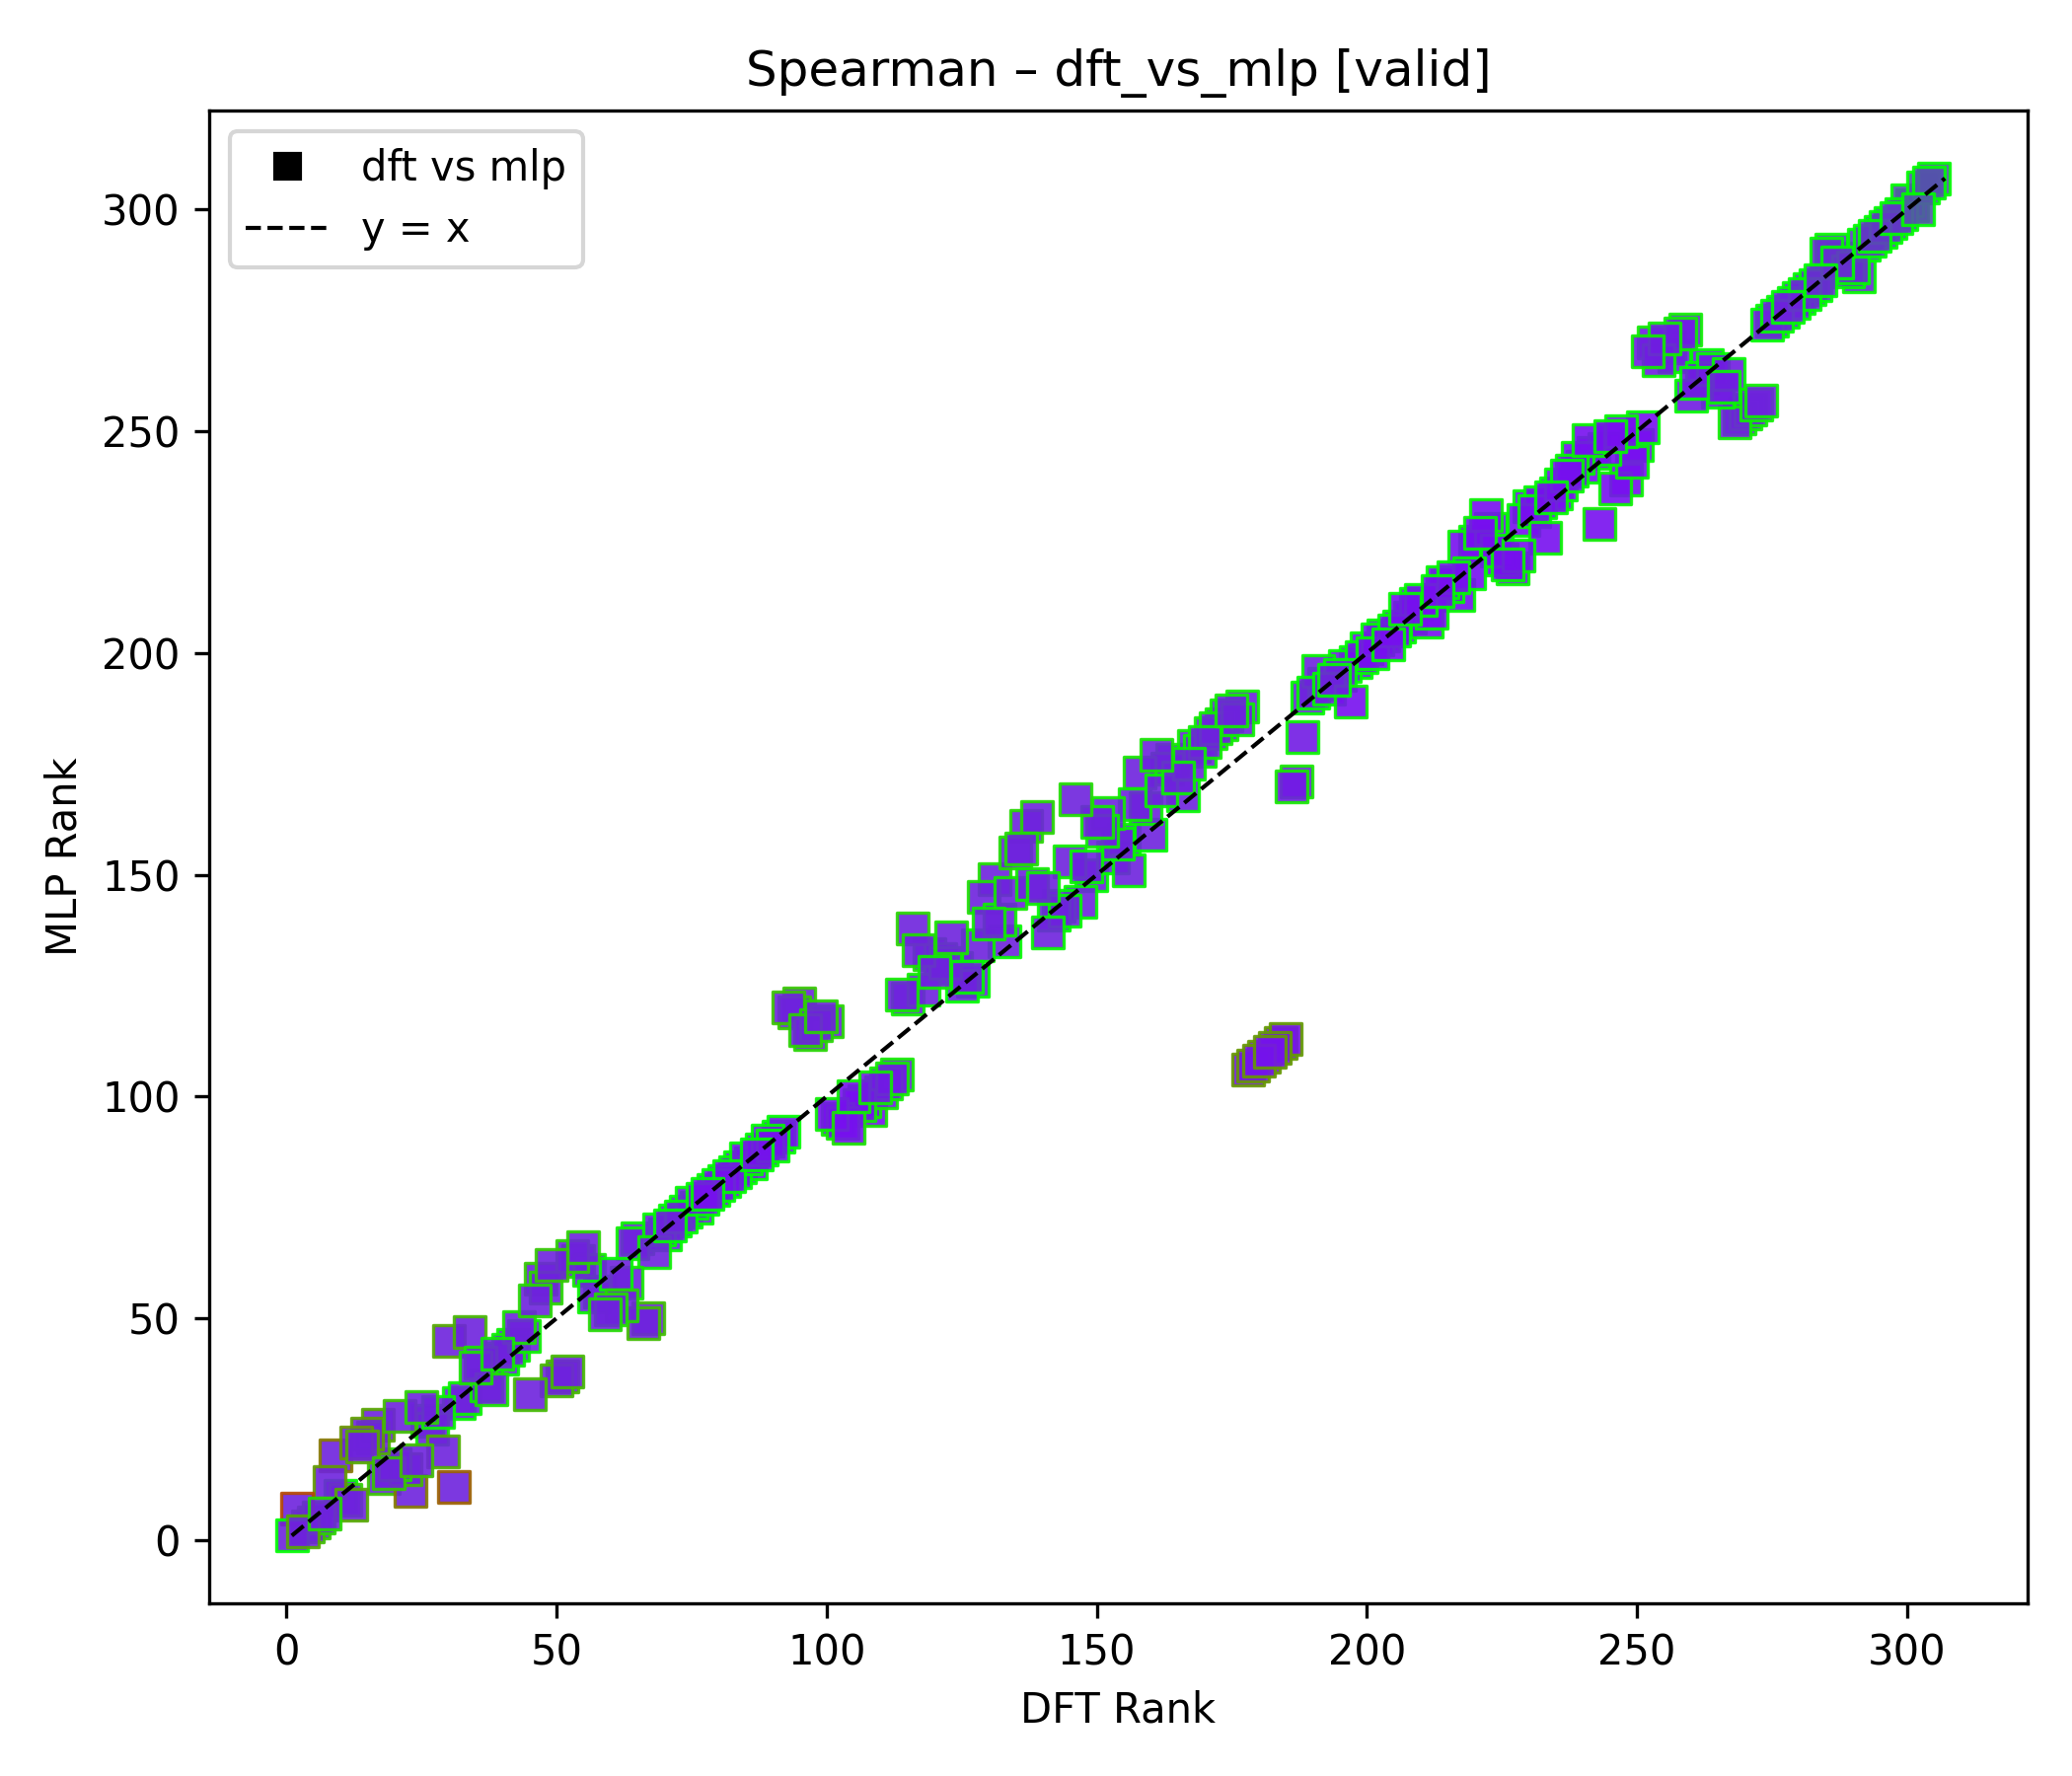
\includegraphics[width=0.7\textwidth]{analysis/plots/results_lower_Si_spearman_unrelaxed_dft_vs_unrelaxed_mlp_valid.png}
    \caption{Spearman rank correlation for $Si$ interfaces, showing strong rank preservation even in lower-$Si$ systems, despite energy disagreement due to geometric artefacts and interfacial strain.}
\end{figure}

Carbon results were geometry-dependent: only three valid $C|Si$ structures with carbon in the lower slab were obtained, and these yielded unreliable results ($\rho = -0.5$), leading to their exclusion from analysis.
However, when carbon appeared in the upper slab ($C|X$), rank correlation was excellent ($\rho = 0.95$), and MAE dropped below $1$ eV. Silicon systems, particularly Si|Ge, showed strong rank correlation but extremely poor energy agreement, while $Ge|Si$ demonstrated improved alignment.
Germanium and tin systems showed robust rank preservation and strong Top-$N$ screening performance across the board.
\begin{table}[h]
    \centering
    \caption{Performance metrics for Si interfaces ($Si$ in upper slab). Lower-slab Si configurations exhibited large energy errors but still maintained reasonable rank correlation (not shown), highlighting geometry sensitivity.}
    \begin{tabular}{lccccc}
        Comparison & Spearman & Kendall & RMSE (eV) & MAE (eV) & Top-10 Overlap \\
        \hline
        \ce{X}|\ce{Si} 100 & 0.989 & 0.931 & 206.397 & 47.779 & 10 \\
        \ce{C}|\ce{Si} 3 & -0.500 & -0.333 & 21.575 & 21.575 & 3 \\
        \ce{Ge}|\ce{Si} 58 & 0.966 & 0.900 & 170.898 & 40.365 & 10 \\
        \ce{Sn}|\ce{Si} 23 & 0.978 & 0.897 & 333.921 & 102.330 & 10 \\
        \ce{Si}|\ce{Si} 16 & 0.956 & 0.846 & 1.251 & 1.147 & 10 \\
    \end{tabular}
\end{table}

Although direct MLP-on-DFT-relaxed structure evaluations (DFT-relaxed MLP) were not included due to computational cost, the study revealed that relaxation and evaluation consistency (e.g. full MLP vs full DFT) influence error, and future cross-evaluation may further clarify error sources.

\subsection{Interface Rank Preservation} \label{section:interface_rank_preservation}

While absolute energy errors between MLP and DFT were large (e.g. RMSE $\approx 189$ eV), they were secondary to the study's goal of rank preservation.
In this context, MLPs effectively captured the energetic hierarchy of Ge and Sn interfaces.
\begin{figure}[h]
    \centering
    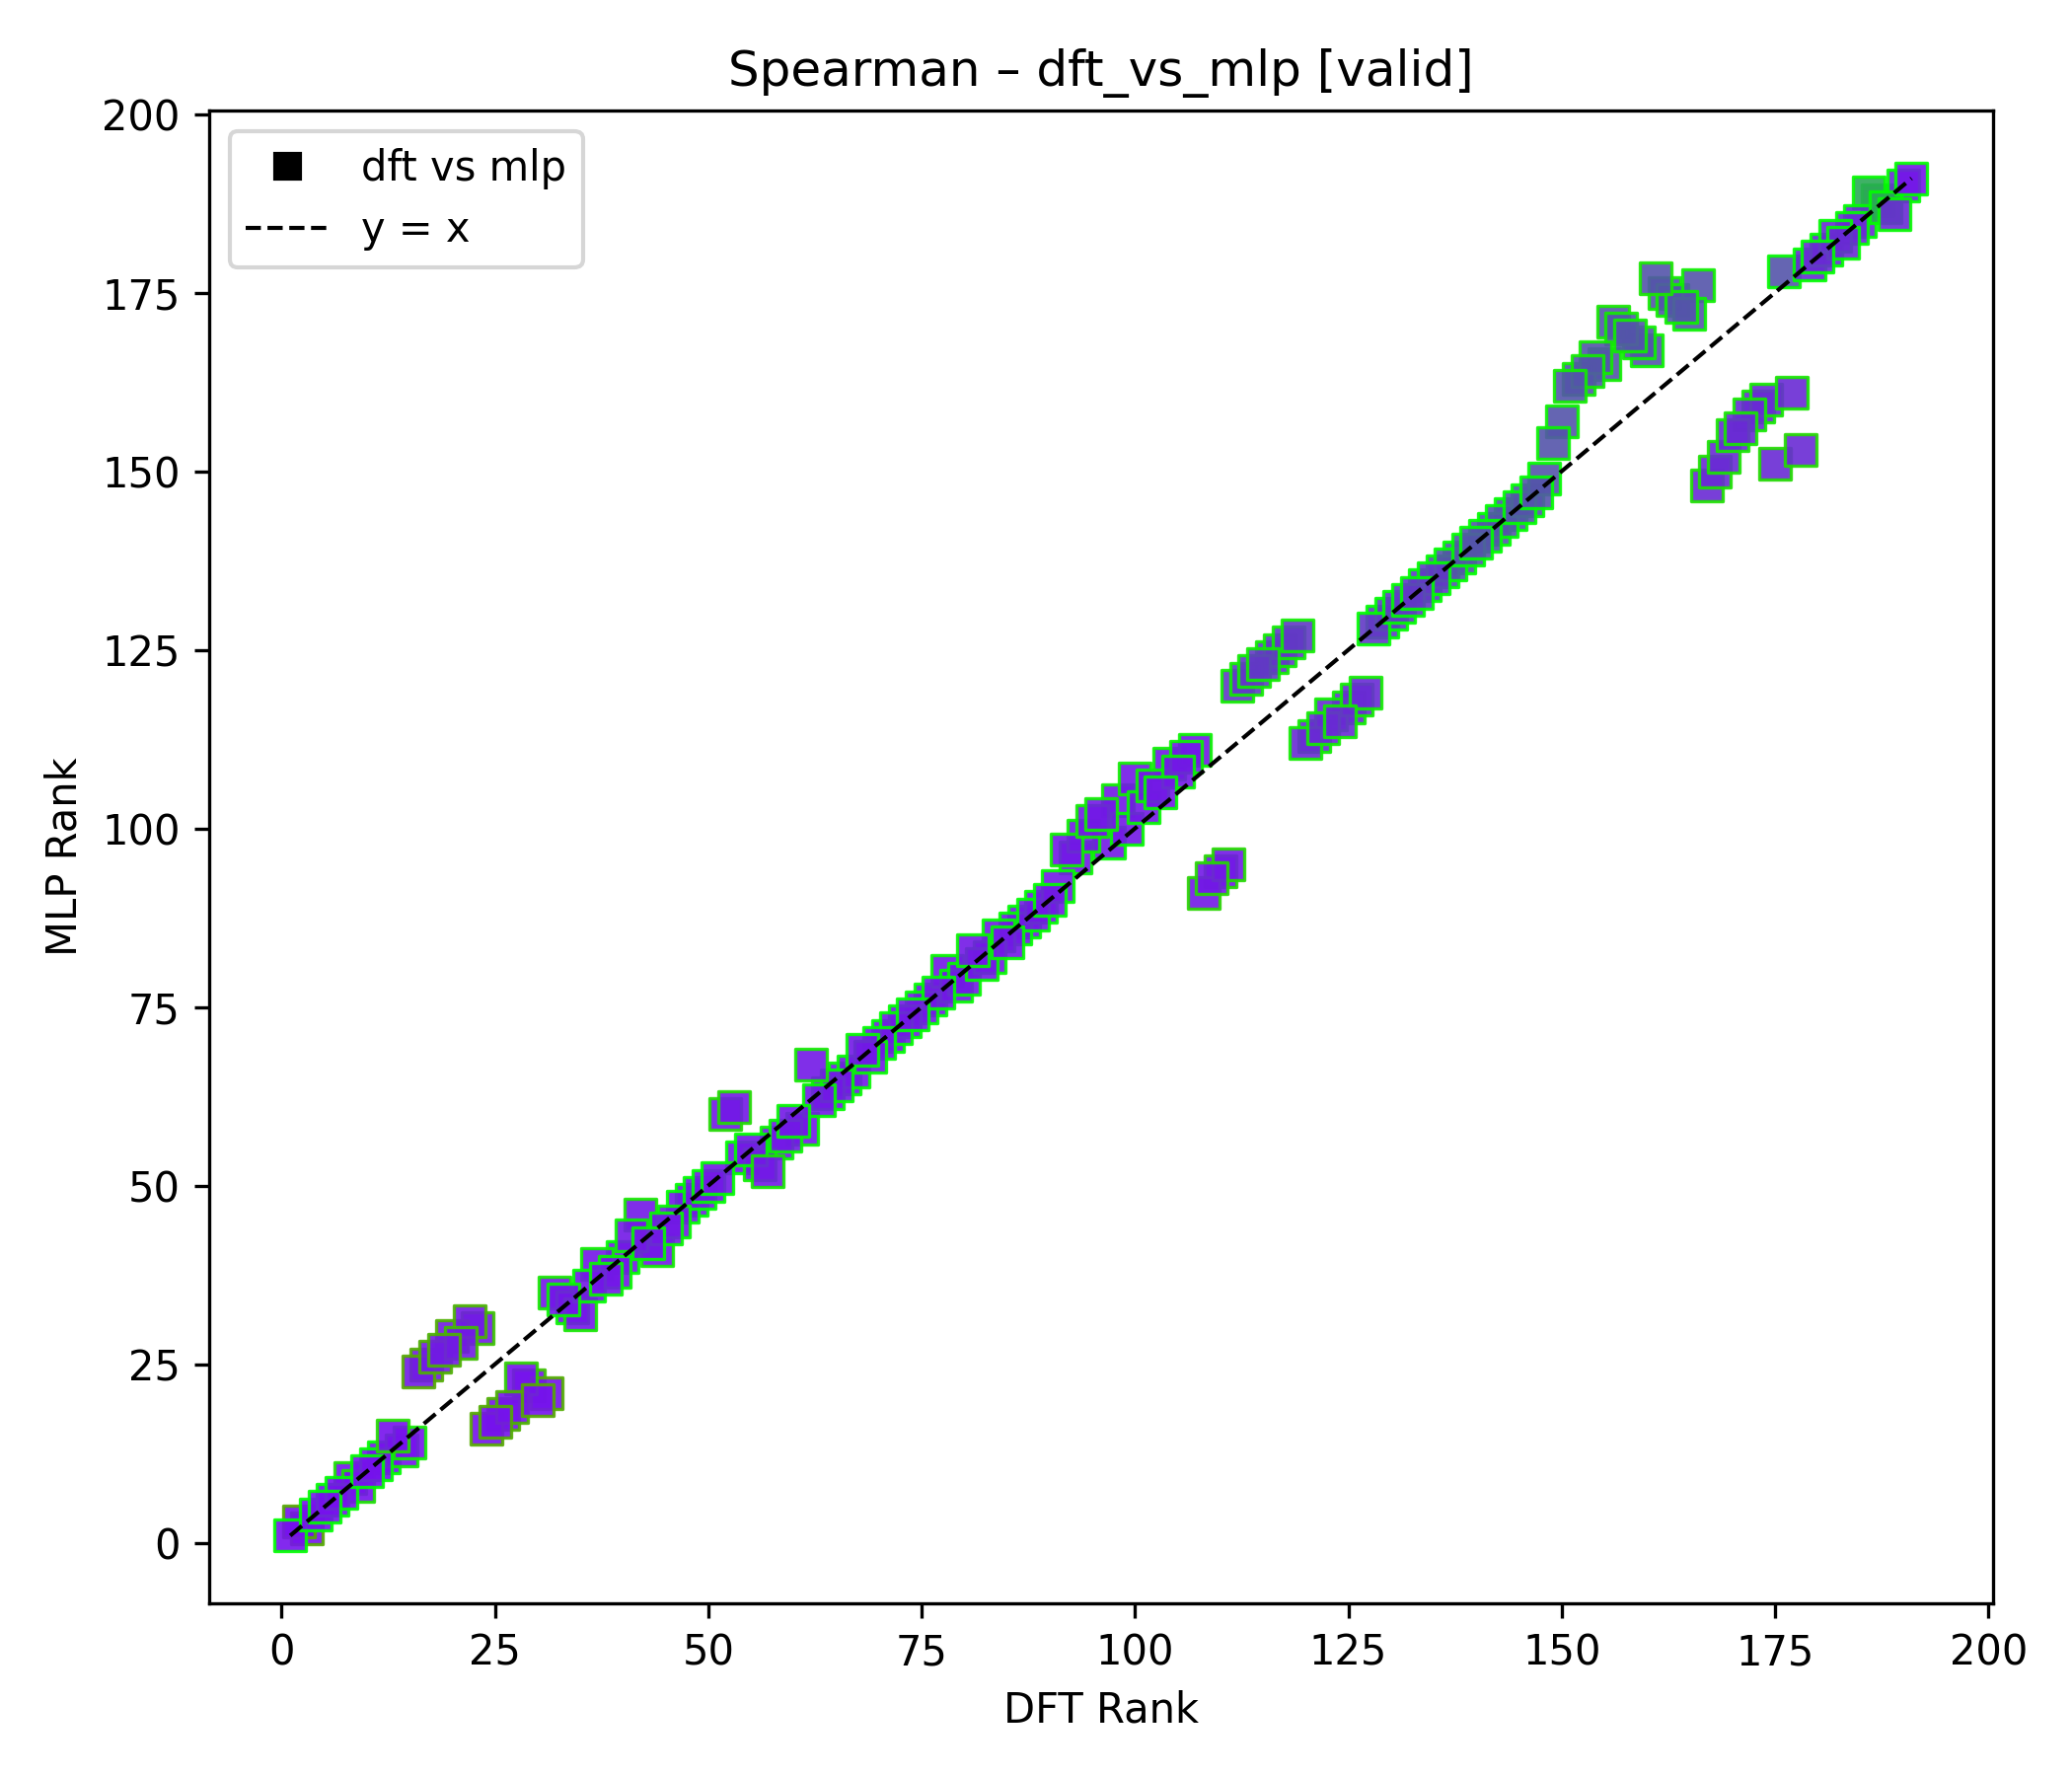
\includegraphics[width=0.7\textwidth]{analysis/plots/results_lower_Ge_spearman_unrelaxed_dft_vs_unrelaxed_mlp_valid.png}
    \caption{Spearman correlation for Ge interfaces.}
\end{figure}

Top-$N$ overlap and rank correlation metrics confirmed that MLPs are useful for screening favourable structures, especially in Ge and Sn systems.
Even when absolute energy values deviated significantly, the identity of the top-ranked configurations was largely preserved, with $8$ out of $10$ matches in many systems.
This supports the use of MLPs like MACE in high-throughput pre-screening pipelines to prioritise candidates for costly DFT relaxation.
\begin{figure}[h]
    \centering
    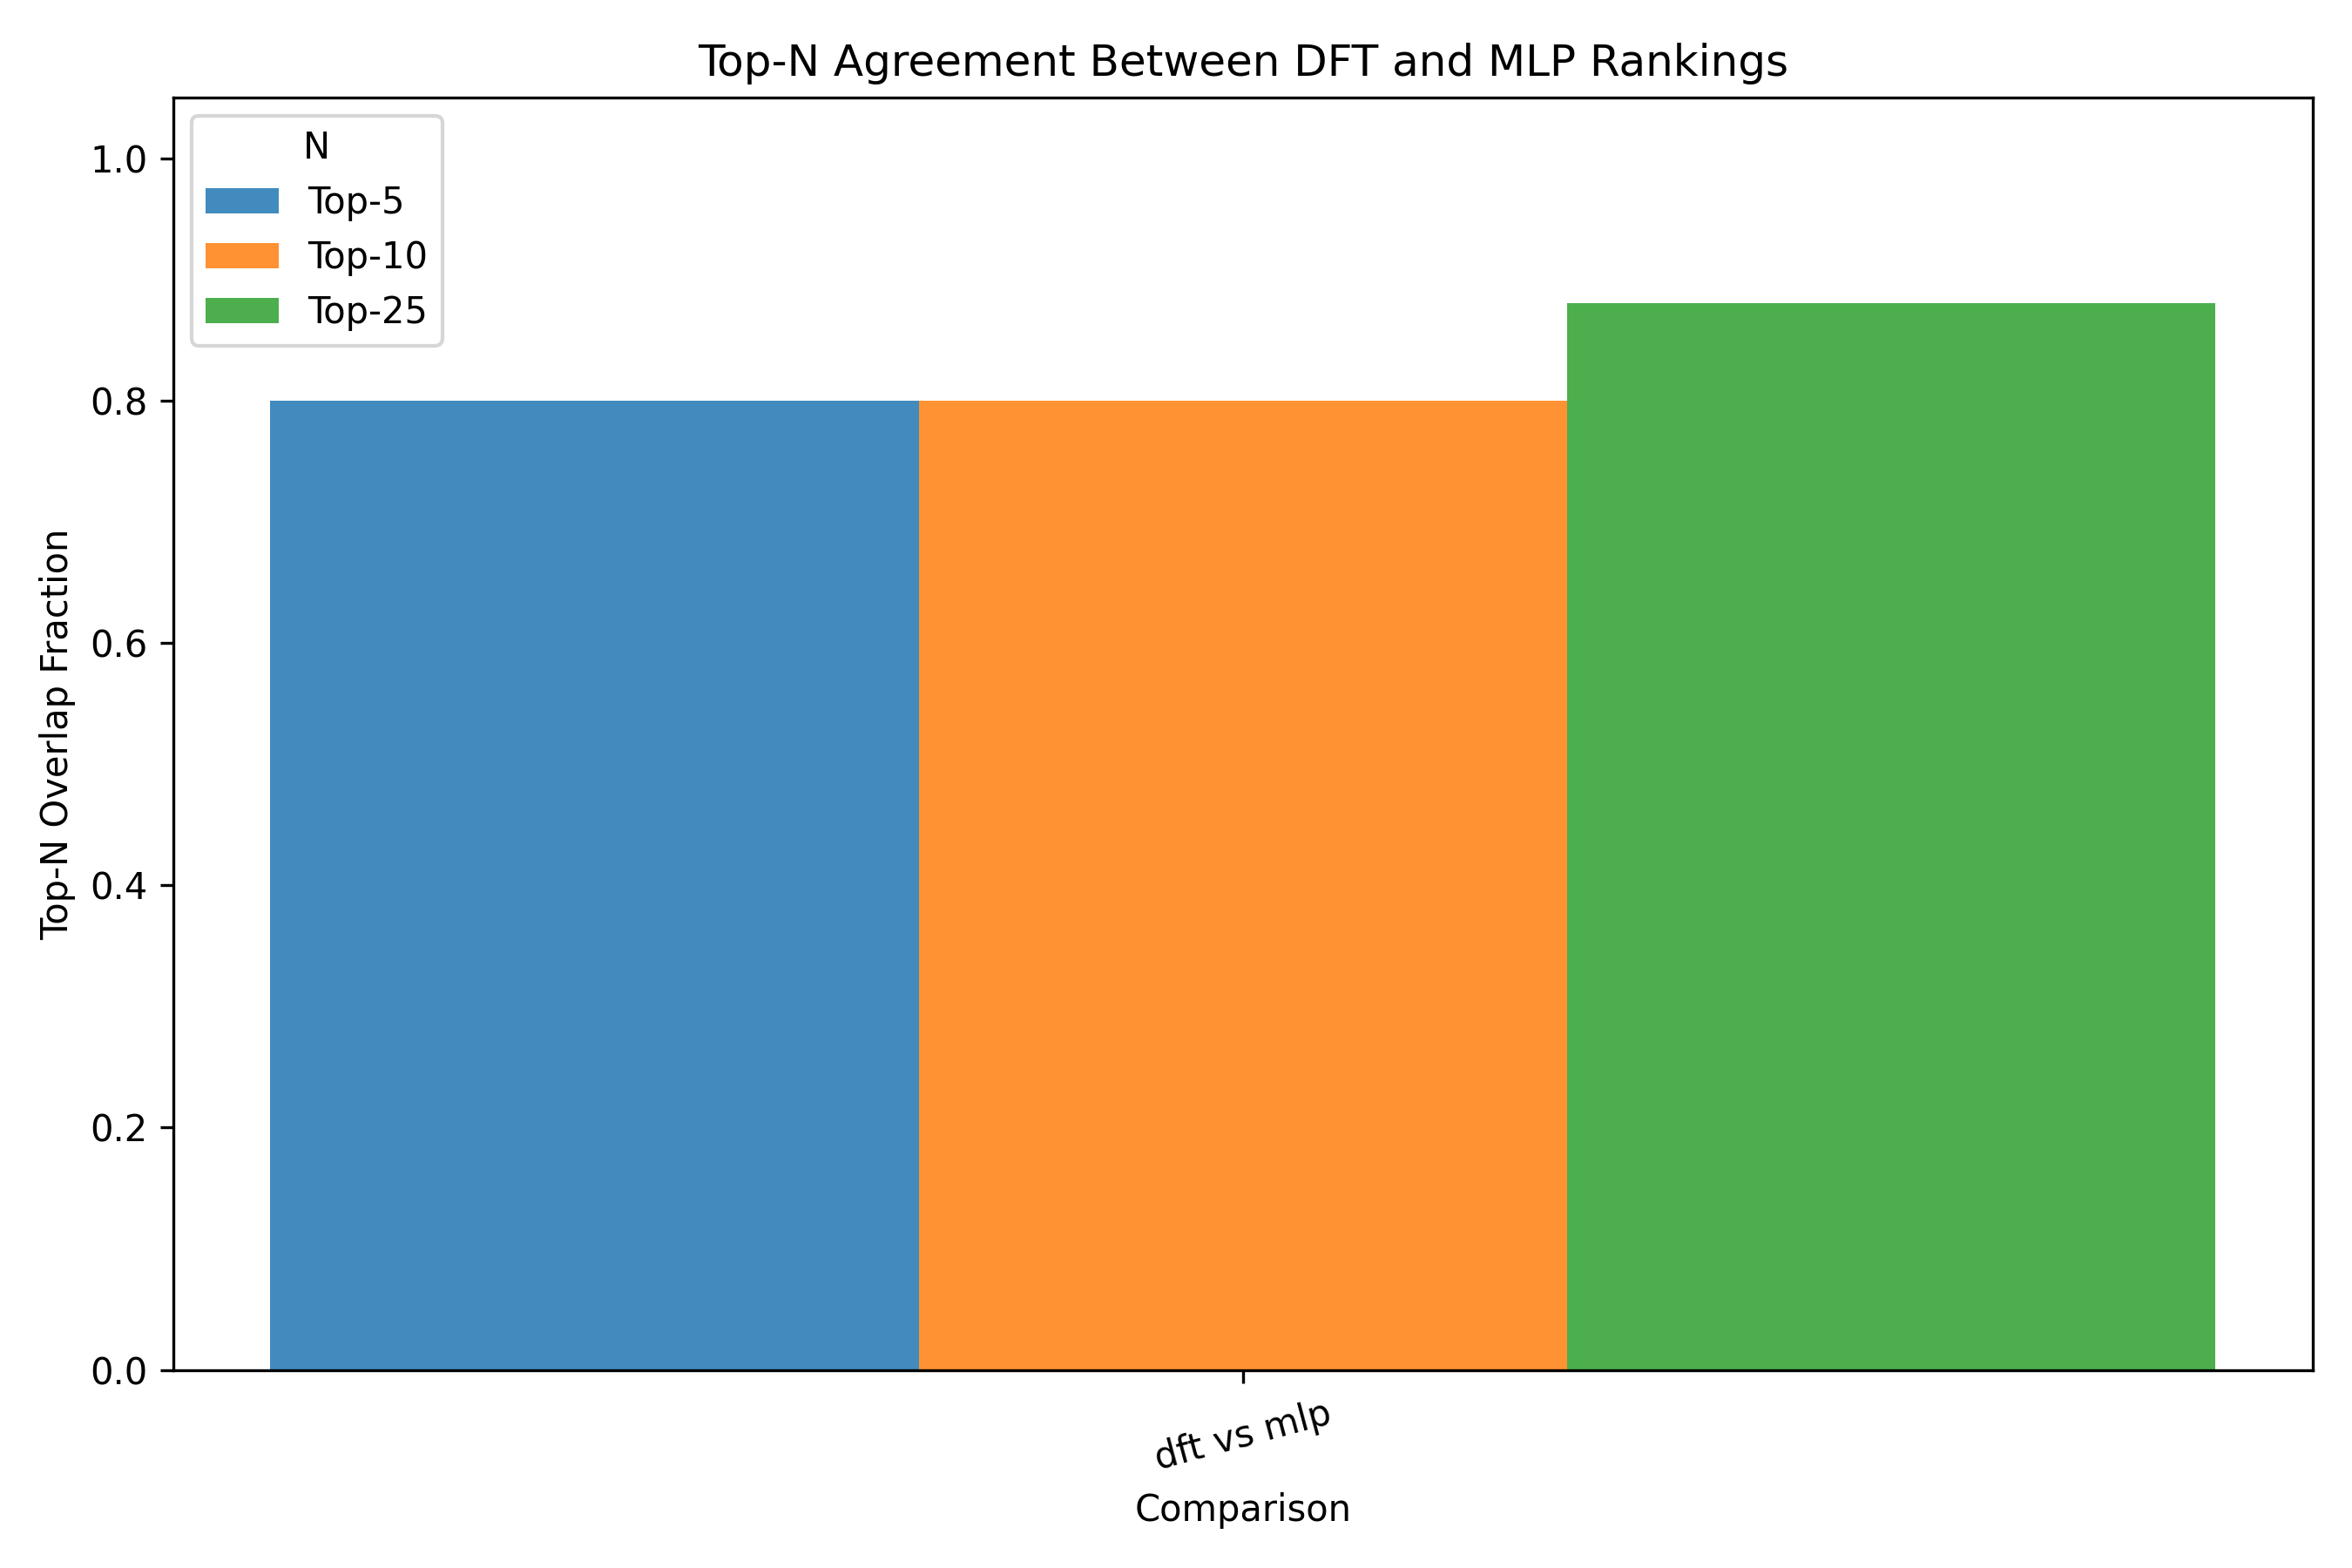
\includegraphics[width=0.7\textwidth]{analysis/plots/results_lower_Si_topn_overlap.png}
    \caption{Top-\textit{N} overlap for Si interfaces.}
\end{figure}

\subsection{Generalisation and Limitations}

MLPs offer significant computational speed advantages and can be reliably used for preliminary screening in systems with well-represented local bonding environments, such as $Ge$, $Sn$, and some $C|X$ combinations.
However, their generalisation is limited in geometrically asymmetric or strained systems, such as $Si|Ge$ or $Sn|Si$, where stacking direction and coordination strongly influence prediction quality.
Without targeted retraining or domain-specific corrections, MLP-based predictions in such cases may be misleading.
\begin{figure}[H]
    \centering
    
\includegraphics[width=1\textwidth]{Upgrade_Report/analysis/plots/results_compute_time_comparison.png}
    \caption{Average compute time per electron versus total electron count for interface structures, comparing DFT (blue) and MLP (orange) energy evaluations. Compute time was measured in walltime seconds on equivalent hardware. DFT exhibits a significantly steeper increase in cost with system size, with a linear trend slope of $1.51 \times 10^{-2}$, compared to just $2.05 \times 10^{-3}$ for MLP—a roughly $7 \times$ slower growth rate. This illustrates the much better scalability of machine-learned potentials for large-scale or high-throughput interface screening.}
    \label{fig:electron_compute_time}
\end{figure}